\documentclass[emulatestandardclasses]{scrartcl}
\usepackage{graphicx}
\usepackage{color}
\usepackage[ngerman]{babel}
\usepackage{hyperref}
\usepackage{fullpage}
\usepackage[utf8]{inputenc}
\usepackage{calc} 
\usepackage{enumitem}
\usepackage{titlesec}
\newcommand{\todo}[1]{\textcolor{red}{TODO: #1}\PackageWarning{TODO:}{#1!}}
\date{\vspace{-3ex}}
\begin{document}

\title{
	\includegraphics*[width=0.75\textwidth]{ErstesSem/images/hu_logo.png}\\
	\vspace{24pt}
	Die Erfahrung der Realität\\durch Widerstand}
\subtitle{\vspace{10pt}Proseminar WS 17/18\\
          Matthias Schlo"sberger\\
          Philosophisches Institut I \\ 
          Humboldt Universit"at zu Berlin}
\author{Lennard Wolf\\
        \small{\href{mailto:lennard.wolf@student.hu-berlin.de}{lennard.wolf@student.hu-berlin.de}}}
\maketitle
\begin{abstract}
Häufig wird Erkenntnistheorie als Versuch der Rechtfertigung von Erkenntnis betrieben. Dass es möglich ist, von der Rechtfertigung einer Erkenntnis zu sprechen, verweist auf ein Problem, das vor allen Fragen der Rechtfertigung geklärt werden sollte. Bevor eine Erkenntnis gerechtfertigt werden kann, muss das in der Erkenntnis Erkannte erfahren werden. Dies, so die Arbeitshypothese des Seminars, gilt auch und insbesondere für die Erfahrung von Realität.
Eine mögliche Antwort auf die Frage, wie die Erfahrung der Realität gemacht wird, lautet: durch die Erfahrung der Widerständigkeit von etwas (der Welt, des Psychischen, des Physischen, des Anderen etc.). Ziel des Seminars ist es, diese Antwort bei einigen für dieses Thema klassischen Autoren zu untersuchen. Besonders wichtig wird es sein, einen klaren Begriff des Widerstands zu entwickeln, der an vielen verschiedenen Phänomenen erläutert werden kann.

\end{abstract}
\newpage

\tableofcontents
%\listoffigures
\newpage


\section{Einf"uhrung\\(19.10.17)}

\begin{itemize}
  \item Moodle-Passwort: Scheler
\end{itemize}


\subsection{Überblick über die Fragestellung}

\begin{itemize}
  \item Realismus vs. Idealismus
  \item Fragestellungen dieser Alternative: Ob wir Zugang zu Realität/Wirklichkeit haben und wenn ja, welchen?
  \item Realisten: Ja.
  \item Idealisten: Die Wirklichkeit wie sie an sich ist können wir nicht erfahren, sondern: das was wir als Wirklichkeit erfahren das ist immer Konstruktion des Subjekts (\emph{subjektiver Idealismus}) oder durch kollektive Konstruktion (\emph{Konstruktivismus})
  \item Essenzaussagen oder Existenzaussagen (was vs. dass) sind gekoppelt an Idealismus vs. Realismus
  \item Matrix: was oder dass Problem
  \item Descartes Ausgangsfrage: Wir müssen alles in Zweifel ziehen. Was bleibt übrig: ego das cogito machen tut (\emph{cogito existo})
  \item Wie können wir von unserer Existenz auf die Existenz der Welt schließen?
  \item Ist die Welt geträumt? Wie unterscheiden wir Traum und Wirklichkeit?
  \item Um zu fragen, ob das Wirklichkeit ist, muss ich mit dem Gegenteil bekannt sein.
  \item Ob das Urteil darüber wahr ist, ist eine andere Frage. (erst danach!)
  \item Klassische Frage: Gibt es Beweise dafür, ob die sogenannte außenwelt existiert?
  \item Übersieht, dass anderer Frage vorgelagert ist: Wie können wir dazwischen unterscheiden?
  \item Philosophie als Fundierungsprojekt! Unterscheidungsfrage ist noch zu klären!
  \item Damit wird die Frage Realismus vs. Idealismus nicht überflüssig! (wie Scheler, Carnap behauptet haben)
  \item Aber: Ändert dieses Fundierungsprojekt überhaupt etwas an der Unterscheidung?
  \item Ob wir in Erfahrungen, durch die wir mit der Unterscheidung vertraut werden, ob das wahr ist, sei erstmal dahingestellt. (macht nichts wenn wir vertauschen, denn wir sind trotzdem mit der Unterscheidung bekannt!)
  \item Dildheim: Über den Grund zur Annahme zur Existenz der Außenwelt 
  \item Repräsentationalismus: Annahme: Zugang zur Welt ist, dass sie vorgestellt ist, dass die Welt in meinem Bewusstsein, dann bedarf es eines Kriteriums dafür, dass die echte Welt 
  \item Naiver, Direkter und Kritischer Realismus
  \item Derealisierung: Die anderen sind da, aber nicht wirklich
  \item Inwiefern können wir uns die ganzen Sinne vorstellen?
  \item Bedeutung der Frage: In welchen Akten unterscheiden wir die Wahrnehmung als wirklich und unwirklich?
  \item Ist das zu kurz gekommen weil wir in erkenntnistheoretischen Fragen uns nur Rechtfertigungen beschäftigt haben und weil wir uns zu sehr an dem "`visozentrischen"' Modell orientiert haben?
  \item In diesem Seminar: Tastsinn wurde eminent vernachlässigt, obwohl dieser zunächst von der Wirklichkeit der Welt überzeugt ist
  \item Aus diesem Widerstand ziehen wir die tiefe Überzeugung, dass die Welt da ist!
  \item Haben Leute mit Derealisierungsproblemen Schwierigkeiten mit dem Widerstand?
  \item Gründen alle Erfahrungen der Welt in Widerständen?
  \item Entfremdungsphänomene: Hier ist jemand nicht mehr in der Lage, Widerstandserfahrungen zu machen.
  \item Vernunfteinsichten helfen nicht weiter! Sie können Problem fixieren, aber nicht lösen.
\end{itemize}

\subsection{Gestaltung des Semesters}

\begin{itemize}
  \item Erster Schritt: Platons Höhlengleichnis - vergegenwärtigen, was das Grundproblem von Realismus/Idealismus ist
  \item Zweiter Schritt: Text, der entscheidender Bezugspunkt Entwicklung des Widerstandsarguments Grund Über den Grund zur Annahme zur Existenz der Außenwelt
  \item Dritter Schritt: Scheler: Hat am schärftsten artikuliert (auch vllt. David Katz ("`Aufbau der Tastwelt"') zur Anregung)
  \item Letztes Drittel: Merleau-Ponty, Waldenfels (responsive Ethik), Psychopathologische Phänomene (Thomas Fuchs (Karls Jaspers Lehrstuhl in Heidelberg))	
\end{itemize}


\newpage
%\section{"Uber den Professor}
%Matthias Schlo"sberger ist Heisenbergstipendiat der Deutschen Forschungsgemeinschaft
%an der Humboldt Universit"at zu Berlin mit dem Forschungsprojekt "`Die Erfahrung der Realit"at durch Widerstand"'.
%
%\begin{figure}[h]
%	\centering
%	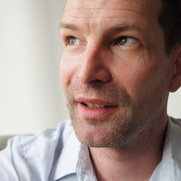
\includegraphics[width=0.3\textwidth]{images/Matthias_Schlossberger.png}
%	\caption{Matthias Schlo"sberger}
%	\label{fig:MS}
%\end{figure}


%\begin{figure}[h]
%	\centering
%	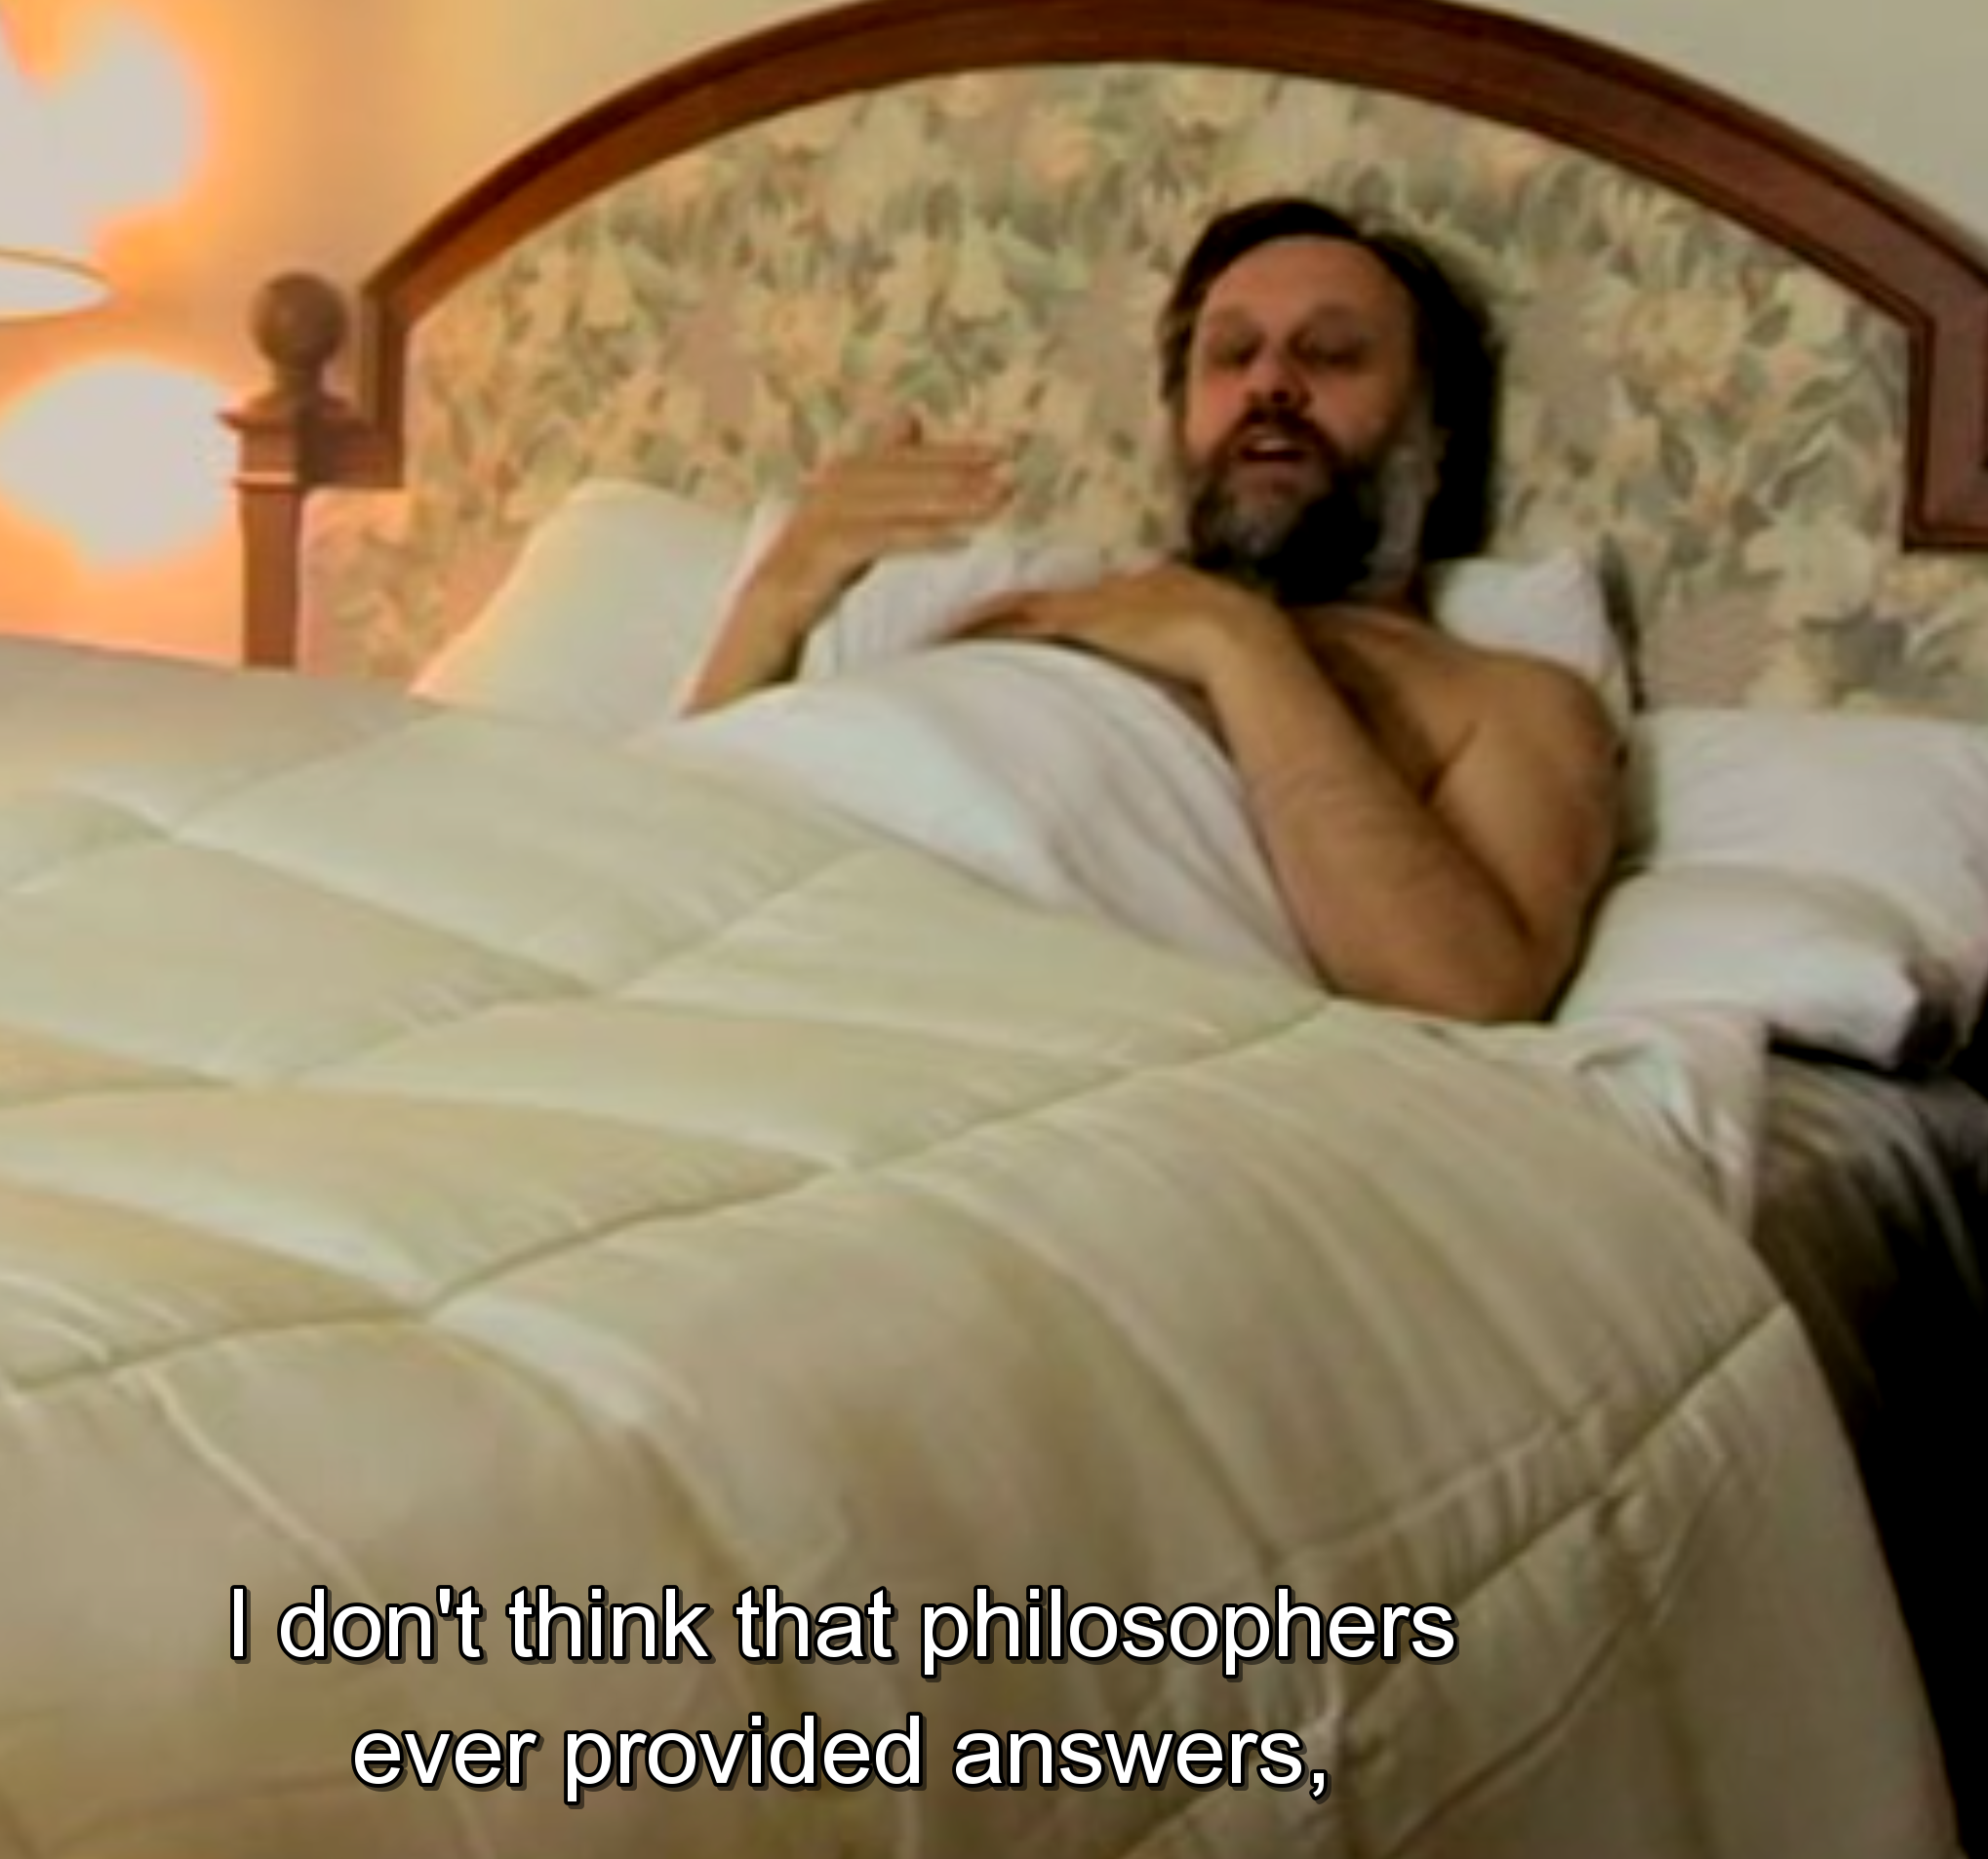
\includegraphics[width=0.5\textwidth]{images/template.png}
%	\caption{Template Bild}
%	\label{fig:template}
%\end{figure}

\end{document}
